\section{Gli attacchi scelti}
Tra gli attacchi presenti nell'ART sono stati analizzati solamente gli evasion attacks per i seguenti motivi:\begin{itemize}
    \item utilizzando un modello preaddestrato ha poco senso andare a implementare i poisoning attacks, in quanto essi agiscono durante la fase di training
    \item gli extraction attacks sono stati esclusi in quanto LearningByCheating è open-source mentre questo tipo di attacchi sono rilevanti quando si ha a che fare
    con algoritmi proprietari
\end{itemize}
Tra gli attacchi analizzati ne abbiamo individuati cinque di particolare interesse:\begin{itemize}
    \item Adversarial Patch,
    \item Spatial Transformation,
    \item HopSkipJump,
    \item Basic Iterative Method,
    \item NewtonFool.
\end{itemize}
\subsection{Adversarial Patch} 
\begin{figure}[h]
    \includegraphics[width=\linewidth]{adversarial_patch.png}
    \caption{adversarial patch\cite{patch}}
    \label{fig:patch}
\end{figure}
In questo attacco si genera una patch che, quando entra nel campo visivo di un classificatore, causa un'errore di misclassificazione. Lo sviluppo dell'attacco è 
indipendente dalla immagine su cui viene generata. La patch generata può essere applicata direttamente alle immagini ma l'utilizzo più interessante è senza dubbio la stampa e l'applicazione di tale patch
ad oggetti fisici. In questo caso la patch potrebbe essere distribuita attraverso internet, stampata, e utiilizzata da un qualsiasi attaccante. Questo attacco è profondamente atipico rispetto
ai normali evasion attacks. La perturbazione è infatti di grandi dimensioni e questo potrebbe sembrare controintuitivo rispetto a ciò che sappiamo di tali attacchi. Ma il vantaggio principale
sta proprio nella sua natura unica: una grande perturbazione è "resistente" anche rispetto ai normali metodi di difesa che si concentrano sulle piccole perturbazioni, ma che possono essere annullate in 
casi così estremi \cite{patch}.
\subsection{Spatial Transformation}
\begin{figure}[h]
    \includegraphics[width = \linewidth]{spat.png}
    \caption{esempi di trasformazioni avversarie\cite{spatial}}
    \label{fig:spat}
\end{figure}
La perturbazione generata è di tipo spaziale. Si cercano i parametri $(\delta u,\delta v,\theta)$ per cui un'immagine ruotata di un angolo $\theta$ e traslata di 
$(\delta u, \delta v)$ pixel viene classificata in modo errato, massimizzando la loss function. Questo tipo di perturbazioni può essere generato in modo "maligno", ma può anche essere causato da perturbazioni naturali(gli oggetti reali
non sempre appaiono perfettamente centrati) \cite{spatial}.
\subsection{HopSkipJump}
\begin{figure}[h]
    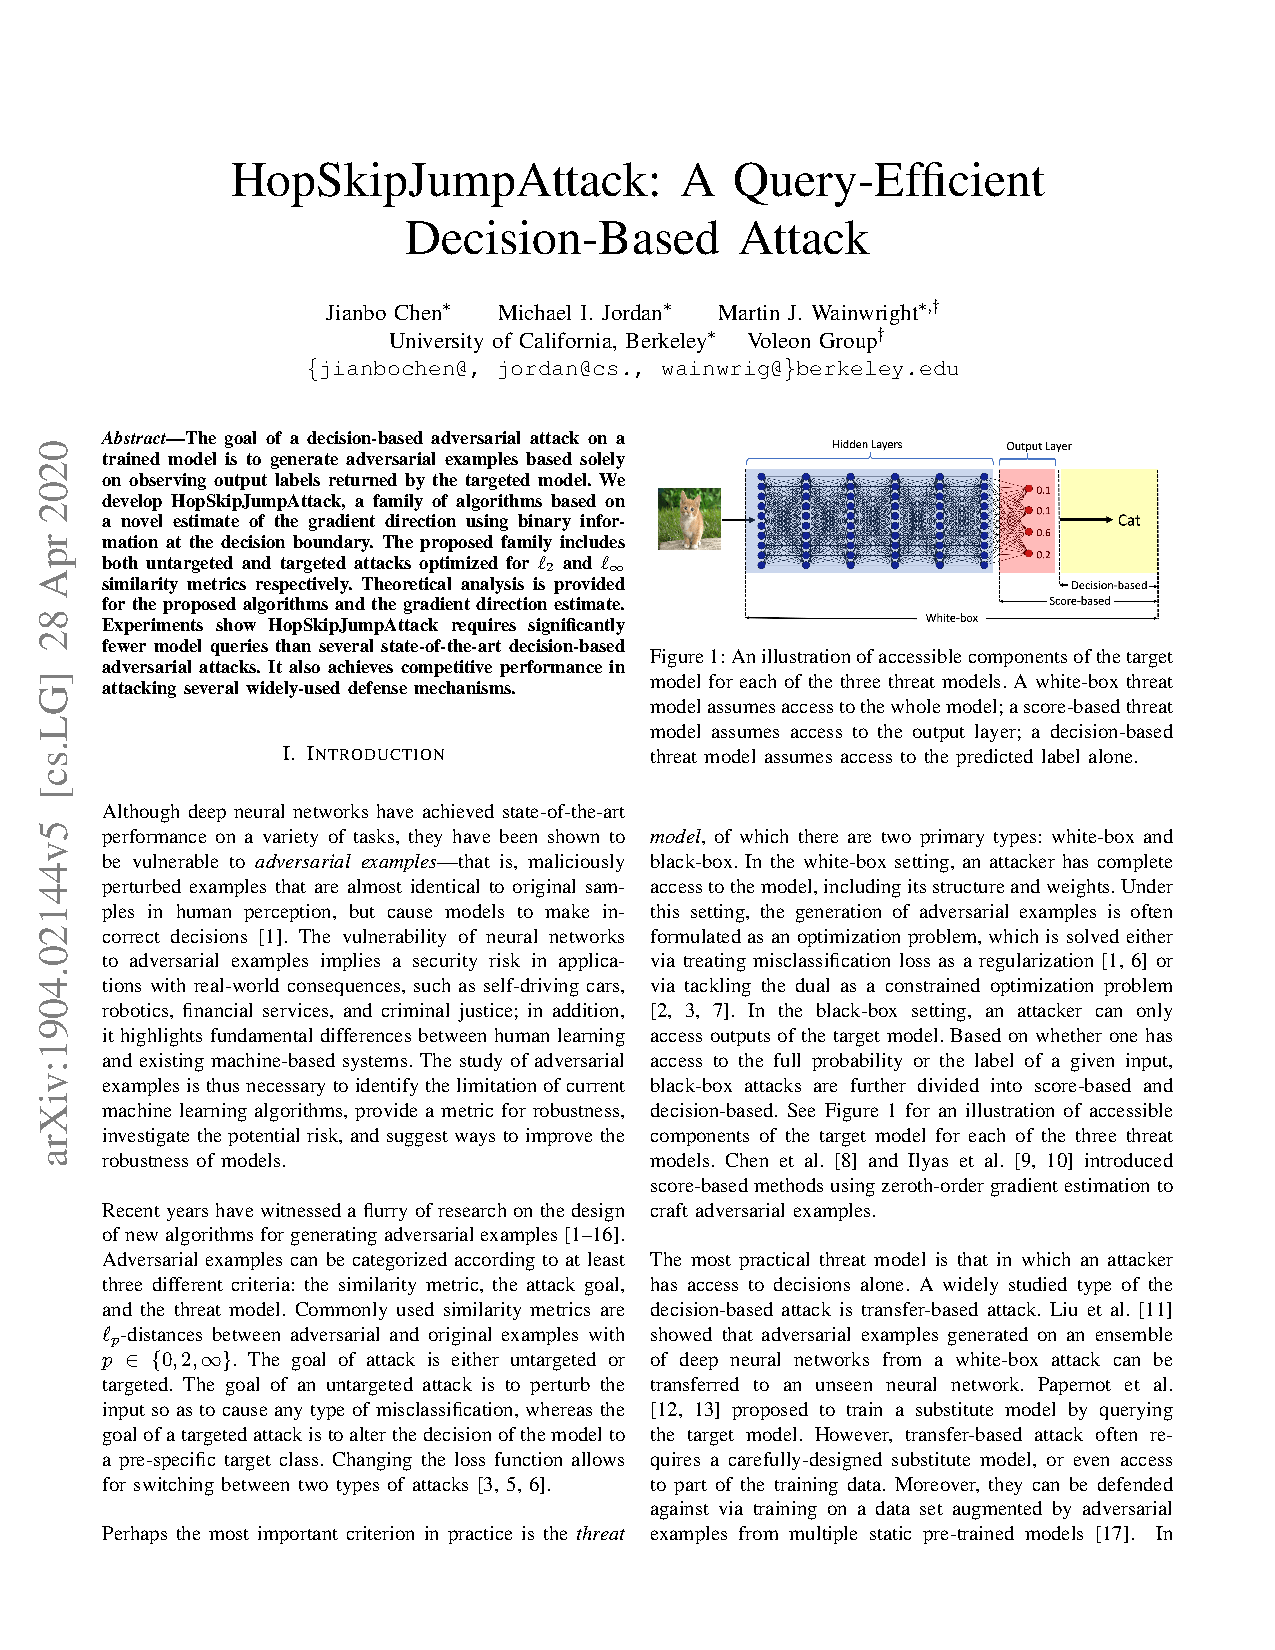
\includegraphics[width=\linewidth]{hop.png}
    \caption{funzionamento dell'hopskipjump\cite{hopskip}}
    \label{fig:hop}
\end{figure}
Parte da una grande perturbazione e punta a ridurla al minimo mantenendo comunque l'errore di classificazione.
La perturbazione viene ridotta attraverso diverse iterazioni di ricerca binaria. Ciascuna iterazione individua una nuova perturbazione valida, più "piccola" della precedente \cite{hopskip}.
\subsection{Basic Iterative Method}
Versione iterativa del Fast Gradient Method. Tale metodo genera una perturbazione risolvendo il problema di massimizzare la loss function con la seguente equazione:

\[X^{adv} = X + \epsilon sign(\nabla _{X}J(X,y_{true}))\]

Nel BIM  questa operazione viene ripetuta per un numero arbitrario di iterazioni, andando a clippare la perturbazione generata ad ogni passo  in modo da restare
all'interno dei limiti predisposti dall'iperparametro $\epsilon$ \cite{bim}.

\[X^{adv}_{0} = X, X^{adv}_{N+1} = Clip_{X,\epsilon}\{ X^{adv}_{N} + \alpha sign(\nabla _{X}J(X^{adv}_{N},y_{true})) \}\]

$\alpha$ indica di quanto è stato modificato un pixel ad ogni passo(in questo caso $\alpha=1$)
\subsection{NewtonFool}

Si assuma che  il classificatore $F(x)$ sia della forma $arg max_l F_s(x)$ e che l'output $F_s$ sia disponibile all'attaccante. Se $F(x_0) = l \in C$ per un qualche  input $x_0$, allora $F^l_s$ è la maggiore probabilità
in $F_s(x_0)$. L'attacco consiste nel trovare un piccolo \textbf{d} per cui $F^l_s(x_0 + d) \approx 0$. L'equazione viene risolta usando il metodo di Newton
per la risoluzione di equazioni non lineari, da cui il nome \cite{newton}.

\subsection{Fattibilità degli attacchi scelti su veicoli a guida autonoma}
Nel contesto di questo lavoro, iniettare un attacco si riduce a modificare il codice del modello LearningByCheating, di cui abbiamo l'accesso completo. 

Nel  mondo reale invece, è necessario prima assumere il controllo della parte del  veicolo che ci permetta di applicare gli attacchi scelti.
Per quattro dei cinque attacchi scelti(hopskipjump,spatial transformation, basic iterative method, newtonfool), iniettarli in un veicolo significa ottenere il controllo del canale
di comunicazione fra camera e l'unità di elaborazione centrale, nella quale è presente il modello decisionale. Così facendo si potrebbero  modificare gli input prima che essi entrino
all'interno del modello stesso.

Questo potrebbe essere realizzato attraverso degli script che sfruttino possibili vulnerabilità del protocollo di comunicazione usato o errori di programmazione.

Per l'attacco Adversarial Patch invece non c'è bisogno  di ottenere il controllo diretto del veicolo. Un attaccante potrebbe generare
una patch in modo indipendente(o addirittura scaricarla da internet) e applicarla sugli oggetti riconosciuti abitualmente da un veicolo(segnali stradali, semafori, fiancate di altre auto ecc.).
\subsection{Attacchi effettivamente iniettati}
Gli attacchi  descritti sono stati tutti iniettati eccetto per Adversarial Patch. La motivazione è di tipo pratico: per poter implementarlo correttamente
avremmo dovuto modificare direttamente dei modelli del simulatore ed applicarci la patch. Nella documentazione di Carla(consultabile a \href{https://carla.readthedocs.io/en/latest/}{\emph{questo indirizzo}})
viene spiegato come aggiungere nuovi modelli. In breve, utilizzando l'editor Unreal va creato un mesh e importato in CARLA insieme 
a una descrizione JSON. Purtroppo abbiamo trovato difficoltà nell'utilizzo dell'editor, soprattutto nell'applicare la patch su un asset preesistente. Abbiamo dunque
ripiegato sul primo approccio, modificando il codice di LearningByCheating e iniettando gli altri quattro attacchi.